\section{Durchführung}
Zunächst wird die Leerlauspannung der zu vermessenden Monozelle direkt mit einem
hochohmigen Voltmeter vermesse, indem dieses direkt mit den Anschlüsssen der Monozelle
verbunden wird, wobei die angezeigte Spannung sowie der Innenwiderstand des
Voltmeters notiert wird.


\noindent Im zweiten Teil wird die Monozelle dann mit einem Ampermeter und einem
verstellbaren Widerstand $\text{R}_a $ in Reihe geschaltet, wobei das Voltmeter
aus dem ersten Teil weiterhin parallel geschaltet wird, um den Spannungsabfall über
die Monozelle zu messen. Diese Schaltung ist auch in Abbildung \ref{fig:schalt2}
dargestellt.
\begin{figure}[H]
  \centering
  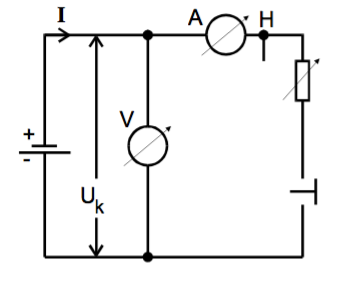
\includegraphics[height=6cm]{schalt2.png}
  \caption{Schaltung der zweiten Messung \cite{skript}}
  \label{fig:schalt2}
\end{figure}
\noindent Dabei wird der Widerstand $\text{R}_a $ zwischen $ 0 - 50 \si{\ohm}$ variiert
und Wertepaare aus dem Strom I und der Spannung $\text{U}_k $ gemessen. \\
\noindent Anschließend wird zusätzlich eine Gleichspannungsquelle mit etwa $\SI{2}{\volt}$
Spannung mehr als die der Monozelle in Reihe in genau entgegengesetzte Richtung
geschaltet, wie in Abbildung \ref{fig:schalt3} zu sehen ist.
\begin{figure}[H]
  \centering
  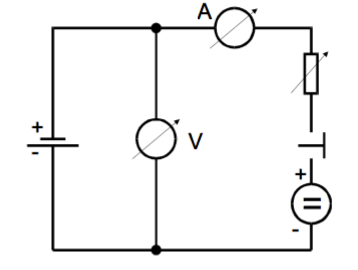
\includegraphics[height=6cm]{schalt3.png}
  \caption{Schaltung der dritten Messung \cite{skript} }
  \label{fig:schalt3}
\end{figure}
\noindent Die Messung erfolgt analog wieder durch Variation des Widerstands und Messung von Strom
und Spannung. \\
\noindent Danach wird die zusätzliche Spannungsquelle wieder ausgebaut und die
Monozele durch einen RC-Generator ersetzt. Auf diesem wird dann eine
Rechteckspannung eingestellt, woraufhin der Widerstand zwischen $ 20-250 \si{\ohm}$
variiert wird und erneut Messwerpaare aus Strom und Spannung am Ampere- und Volt-Meter
abgelesen werden.
Schlussendlich wird diese Messung noch mit einer Sinusspannung wiederholt, wobei
der Wertebereich des Widerstands diesmal zwischen $0.1 - 5 \si{\kilo\ohm}$ liegen
soll.
